% !TEX root = ../thesis.tex

\graphicspath{{ch-math/figures/}}

\chapter{Mathematical Methods}\label{ch:math}


\section{Manifold Learning Based on Laplace Operators} \label{sec:manifold_learning}

{\em This section is currently being prepared for publication along with \chap~\ref{ch:harmonics}}.
%Although data from dynamical systems is often high-dimensional, since it is collected at the microscale, the macroscale dynamics often evolve to a low-dimensional description.
%
%In such cases, the high-dimensional microscale data is restricted to a low-dimensional manifold embedded in the high-dimensional space, and extracting a parametrization of this manifold corresponds to parametrizing the low-dimensional, macroscale dynamics.
%

Let $\data(1), \dots, \data(m) \in \mathbb{R}^\highdim$ denote $\ndata$ observations sampled from a dynamical system.
%
We assume the $\highdim$-dimensional observations $\data(i)$ lie on a $\lowdim$-dimensional manifold $\manifold$, where $\lowdim < \highdim$.
%
We therefore consider the problem of parametrizing the continuous $d$-dimensional manifold $\manifold$ embedded in $\mathbb{R}^\highdim$ from data.
%
For linear hyperplanes, the principal axes parametrize the manifold.
%
However, in the case when the manifold is nonlinear, the set of coordinates is not readily apparent.
%
By using a particular manifold learning technique based on the construction of a Laplace operator, namely, diffusion maps, we will show how to extract a $\lowdim$-dimensional parametrization of the observations which is consistent with the geometry of the manifold \cite{Belkin2003, coifman2005geometric, singer2008non}.

\subsection{Eigenfunctions of the Laplace-Beltrami operator}

\begin{figure}[t]
\centering
\begin{subfigure}{0.3\textwidth}
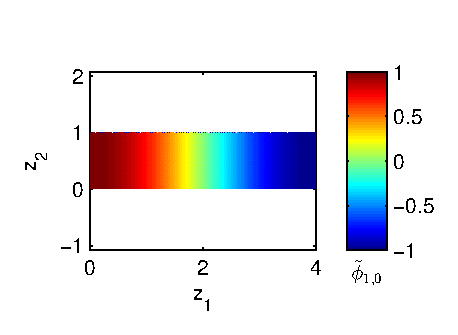
\includegraphics[width=\textwidth]{ch-harmonics/figures/strip_cnts1}
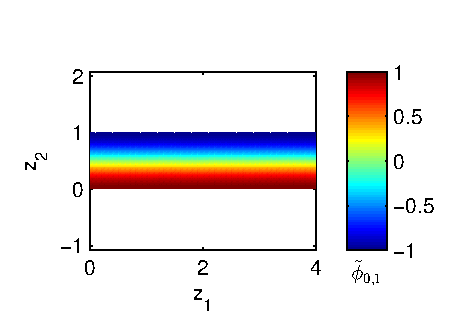
\includegraphics[width=\textwidth]{ch-harmonics/figures/strip_cnts2}
\caption{}
\label{subfig:strip_efuncs}
\end{subfigure}
%
\begin{subfigure}{0.3\textwidth}
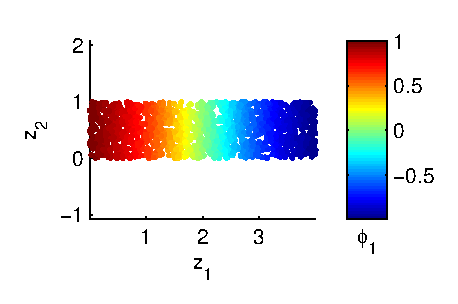
\includegraphics[width=\textwidth]{ch-harmonics/figures/strip_discrete1}
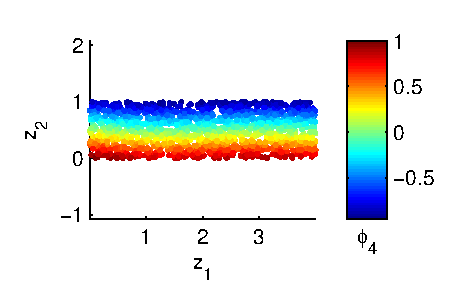
\includegraphics[width=\textwidth]{ch-harmonics/figures/strip_discrete4}
\caption{}
\label{subfig:strip_evecs_uniform}
\end{subfigure}
%
\begin{subfigure}{0.3\textwidth}
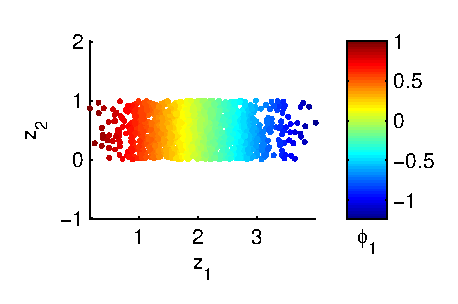
\includegraphics[width=\textwidth]{ch-harmonics/figures/strip_nonuniform1}
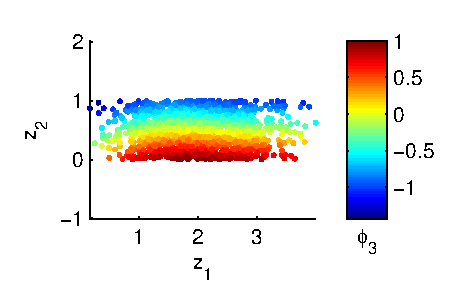
\includegraphics[width=\textwidth]{ch-harmonics/figures/strip_nonuniform2}
\caption{}
\label{subfig:strip_evecs_nonuniform}
\end{subfigure}
%
\caption[Eigenfunctions of the Laplace-Beltrami operator on a two-dimensional strip]{(a) Two-dimensional continuous strip colored by the eigenfunctions $\tilde{\phi}_{1, 0} = \cos \left( {\pi z_1}/{L_1} \right)$, and $\tilde{\phi}_{0, 1} = \cos \left( {\pi z_2}/{L_2} \right)$. (b) Two-dimensional strip with uniform sampling colored by the first and fourth (non-trivial) eigenvectors of the discrete Laplacian. (c) Two-dimensional strip with data sampled from a Gaussian distribution in $z_1$ and sampled uniformly in $z_2$, colored by the first and third (non-trivial) eigenvectors of the discrete Laplacian. Note that in all cases we uncover parametrizations which are one-to-one with $z_1$ and $z_2$.}
\end{figure}

In recent years, it has been noted that the eigenfunctions of the \emph{continuous} Laplace-Beltrami operator provide ``good" coordinates for a manifold \cite{jones2008}.
%
Thus, we start by considering a continuous setting where rigorous analysis is available for specific examples.
%
%Using such an example, we will show that the existence of repeated eigendirections is inherent to the manifold learning setup based on Laplace operators, and that the identification of the unique eigendirections is nontrivial.
%%
%The existence of these challenges in the continuous setting implies that, even in the limit of infinite data, such repeated eigendirections still pose a problem for analysis.
%
To illustrate why these eigenfunctions provide appropriate coordinates, consider a two-dimensional strip with edge lengths $L_1$ and $L_2$.
%
The eigenvalues of the Laplace-Beltrami operator with Neumann boundary conditions are given by
\begin{equation} \label{eq:evals}
\tilde{\lambda}_{k_1, k_2} = \left( \frac{k_1 \pi}{L_1} \right)^2 + \left( \frac{k_2 \pi}{L_2} \right)^2
\end{equation}
for $k_1, k_2 = 0, 1, 2, \dots$,
and the corresponding eigenfunctions are
\begin{equation} \label{eq:efuncs}
\tilde{\phi}_{k_1, k_2} = \cos \left( \frac{k_1 \pi z_1}{L_1} \right) \cos \left( \frac{k_2 \pi z_2}{L_2} \right)
\end{equation}
where $z_1$ and $z_2$ denote the two coordinates of the strip \cite{singer2008non}.
%
We note that the eigenfunctions $\tilde{\phi}_{1, 0} = \cos \left( {\pi z_1}/{L_1} \right)$ and $\tilde{\phi}_{0, 1} = \cos \left( {\pi z_2}/{L_2} \right)$ are one-to-one with the $z_1$ and $z_2$ coordinates, respectively, and therefore yield a parametrization of the underlying manifold (see Figure~\ref{subfig:strip_efuncs}).
%
Furthermore, the corresponding eigenvalues $\tilde{\lambda}_{1,0}$ and $\tilde{\lambda}_{0,1}$ provide a measure of $L_1$ versus $L_2$: as the ratio between $L_1$ and $L_2$ increases, the gap between $\tilde{\lambda}_{1,0}$ and $\tilde{\lambda}_{0,1}$ also increases (this will be discussed further in Section~\ref{sec:relative_lengths}).
%
%The analytic form of the eigenfunctions in \eqref{eq:efuncs} illustrates the two issues we address in this paper.
%%
%First, $z_1$ and $z_2$ are not necessarily decoupled in subsequent eigenfunctions, and a proper parameterization of the manifold is not necessarily given by the $d$ eigenfunctions associated with the smallest $d$ eigenvalues.
%% TODO: address this in later section
%%
%Second, eigenfunctions with $k_1+k_2 \ge 2$ do not describe any additional directions along the strip; we will refer to these as ``repeated eigendirections,'' and we will refer to the eigenfunctions with $k_1+k_2 =1$ as ``unique eigendirections.'' 
%%
%We note that, although the eigenfunctions can only be written analytically for very special cases, it has been observed empirically that the eigenfunctions often provide appropriate coordinates to parametrize more complex, nonlinear manifolds.
%%
%In addition, this problem of repeated eigendirections arises for more complex manifolds with more than two variables.


\subsection{Discrete approximation of the Laplace-Beltrami operator: diffusion maps} \label{sec:dmaps}

In most applications, we are not given a description of the continuous manifold.
%
Instead, we are given data {\em sampled} from the underlying manifold, and the parameterization of the manifold needs to be uncovered from the data.
%
It was shown in \cite{coifman2006geometric} that, in the limit of infinite data, this discrete Laplacian matrix constructed from data converges pointwise to the continuous Laplace-Beltrami operator on the manifold.
%
As a result, the eigenvectors of the discrete Laplacian approximate the eigenfunctions of this continuous operator.

Given observations $\data(1), \dots, \data(m) \in \manifold$, we first construct the weight matrix $\mathbf{W} \in \mathbb{R}^{\ndata \times \ndata}$, with
\begin{equation} \label{eq:W} 
\mathbf{W}_{ij} = \exp \left( -\frac{\|\data(i) - \data(j) \|^2}{\dmeps^2} \right), \ i,j=1,\ldots,\ndata,
\end{equation}
where $\| \cdot \|$ denotes the appropriate norm for the observations, and $\dmeps$ is a characteristic distance between the observations.
%
Note that $\dmeps$ induces a notion of locality: if $\|\data(i) - \data(j) \| \gg \dmeps$, then $\mathbf{W}_{ij}$ is negligible.
%
Therefore, we only need our metric to be informative within a ball of radius $\dmeps$.
%
Points less than $\dmeps$ apart are thus considered ``close'' and points farther than $\dmeps$ apart are considered ``far away''.
%
The kernel's scale $\dmeps$ can be chosen using several heuristics \cite{rohrdanz2011determination, coifman2008graph}; we often take $\dmeps$ to be the median of the pairwise distances between the data points.
%
We then construct the diagonal matrix $\mathbf{D} \in \mathbb{R}^{\ndata \times \ndata}$, with $\mathbf{D}_{ii} = \sum_j \mathbf{W}_{ij}$, and form the matrix $\widetilde{\mathbf{W}} = \mathbf{D}^{-\alpha} \mathbf{W} \mathbf{D}^{-\alpha}$, where $0 < \alpha < 1$. 
%
Next, we construct the diagonal matrix $\widetilde{\mathbf{D}} \in \mathbb{R}^{m \times m}$, with $\widetilde{\mathbf{D}}_{ii} = \sum_j \widetilde{\mathbf{W}}_{ij}$, and the matrix $\mathbf{A}  = \widetilde{\mathbf{D}}^{-1} \widetilde{\mathbf{W}}.$

If the data $\data(1), \dots, \data(m)$ are sampled from $\manifold$ with some density $q$, then, for $\dmeps \rightarrow 0$ and $\ndata \rightarrow \infty$ (with the appropriate rates), the discrete matrix convergences to the following continuous limit operators with Neumann boundary conditions \cite{coifman2006geometric}
\begin{equation} \label{eq:limiting_operator}
\begin{aligned}
\frac{1}{\dmeps^2}(\mathbf{I}-\mathbf{A}) \phi &\rightarrow \nabla^2 \phi - 2\nabla U \cdot \nabla \phi, &&\alpha = 0 \\
\frac{1}{\dmeps^2}(\mathbf{I}-\mathbf{A}) \phi &\rightarrow \nabla^2 \phi - \nabla U \cdot \nabla \phi, &&\alpha = 1/2 \\
\frac{1}{\dmeps^2}(\mathbf{I}-\mathbf{A}) \phi &\rightarrow \nabla^2 \phi, &&\alpha = 1
\end{aligned}
\end{equation}
where $U = - \log q$.
%
The different limit operators, depending on the choice of $\alpha$, imply that nonuniform sampling on the manifold may have different effects. 
%
In subsequent chapters, we will use the $\alpha=0$ embedding unless otherwise noted. 
%
Note that by setting $\alpha=1$, one can factor out the density effects in the weight matrix, and the discrete Laplacian matrix approaches the Laplace-Beltrami operator on the manifold $\manifold$.
%
The eigenvectors $\phi_0, \phi_1, \dots, \phi_{\ndata-1}$ of $\mathbf{A}$ approximate the eigenfunctions of the Laplace-Beltrami operator on $\manifold$,
and the eigenvalues $\lambda_0, \lambda_1, \dots, \lambda_{\ndata-1}$ of $\mathbf{A}$ are related to the eigenvalues of the continuous operator by
\begin{equation} \label{eq:evals_relationship}
\lambda_k = \exp \left( -\frac{\epsilon^2}{4} \tilde{\lambda}_{k_1, k_2}  \right).
\end{equation}
%
As discussed previously, the eigenfunctions provide a parametrization of the manifold, such that $\phi_{j}(i)$ yields the $j^{th}$ embedding coordinate for $\data(i)$.
%
The standard diffusion maps embedding incorporates eigenvalue weights \cite{coifman2005geometric, coifman2006geometric},
%
\begin{equation} \label{eq:dmaps_embed_full}
\data(i) \mapsto 
\begin{pmatrix}
\lambda_1^\tau \phi_1(i) \\
\lambda_2^\tau \phi_2(i) \\
\vdots \\
\lambda_{\ndata-1}^\tau  \phi_{\ndata-1}(i)
\end{pmatrix}
\end{equation}
%
where we order the eigenvectors such that $|\lambda_0| \ge |\lambda_1| \ge \dots \ge |\lambda_{m-1}|$, and $\tau \ge 0$ is a parameter (in our examples, we will take $\tau=0$, which corresponds to the Laplacian Eigenmaps formulation).
%
Because the matrix $\mathbf{A}$ is row-stochastic ($\sum_j \mathbf{A}_{ij} = 1$),  $\lambda_0 = 1$ and $\phi_0$ is a trivial constant vector.
%
The distance induced by this embedding is called the standard diffusion distance,
%
\begin{equation}
D^2_\tau(z(i), z(j)) = \sum_{k=1}^{m-1} \lambda_k^{2 \tau} \left( \phi_k(i) - \phi_k(j)  \right)^2.
\end{equation}
%
The diffusion maps embedding therefore projects the data into a space where the Euclidean distance is equivalent to the diffusion distance. 
%
If the eigenvalues exhibit a spectral gap, where $|\lambda_1| \ge |\lambda_2| \ge \dots \ge |\lambda_\lowdim | \gg |\lambda_{\lowdim+1} | \ge \dots \ge |\lambda_{\ndata-1}|$, then one can embed the data in the first $\lowdim$ eigenvectors, 
\begin{equation} \label{eq:dmaps_embed_reduced}
\data(i) \mapsto 
\begin{pmatrix}
\lambda_1^\tau \phi_1(i) \\
\lambda_2^\tau \phi_2(i) \\
\vdots \\
\lambda_{\lowdim}^\tau  \phi_{\lowdim}(i)
\end{pmatrix}
\end{equation}
%
while still approximately retaining the diffusion distance. 

Figures~\ref{subfig:strip_evecs_uniform}--\ref{subfig:strip_evecs_nonuniform} shows data sampled from a strip, colored by eigenvectors of $\mathbf{A}$.
%
In cases of both uniform and nonuniform sampling, the selected eigenvectors are one-to-one with $z_1$ and $z_2$, and thus parametrize the manifold.
%
However, we briefly note that the two diffusion maps coordinates which parameterize the manifold are not guaranteed to be the first two eigenvectors.
%
This is the issue of ``repeated eigendirections,'' where some eigenvectors are higher harmonics of previous eigenvectors and do not capture any new directions in the data; we will discuss this issue in more detail in \chap~\ref{ch:harmonics}. 
%
%TODO: maybe we can put here the new figures for the different values of $\alpha$ instead of these figures.
%
Although we have considered a very simple example of a two-dimensional strip for illustrative purposes, common practice is to use these tools for high-dimensional, nonlinear data sets.

%From the previous section, we know that the eigenfunctions with $(k_1, k_2) =(1, 0)$ and $(k_1, k_2) =(0, 1)$ provide embedding coordinates for the manifold; these two eigenfunctions are both uncoupled and not repeated.
%%
%From \eqref{eq:evals}, we see that sorting the eigenvectors by the magnitude of the corresponding eigenvalues implies that these two eigenvectors are guaranteed to appear before any coupled or repeated eigendirections.
%%
%However, these eigenvectors are {\em not} guaranteed to appear as the first two (non-trivial) eigenvectors, as harmonics of the first eigendirection (i.e., $\cos \left( n \pi z_1 / L_1 \right)$ with $n > 1$) could appear before the second.
%%
%We note that, in contrast to our simple illustrative example, for most data sets of interest, the coordinates for the underlying manifold are unknown and cannot easily be obtained from the coordinates of the original data, and identifying which eigenvectors correspond to unique eigendirections is nontrivial.




%\section{Diffusion maps} \label{sec:dmaps}
%
%Diffusion maps is an unsupervised, nonlinear data mining algorithm. 
%%
%Given $\ndata$ data points $\data(1), \dots, \data(\ndata)$ (typically vectors in a high-dimensional vector space) which lie on a lower-dimensional manifold $\manifold$, the aim of diffusion maps is to uncover a parameterization $f(\data)$ of the data which captures the notion of locality with respect to the manifold: points that are ``close" in the original space should also be ``close" in the coordinates $f$.
%%
%%From pairwise distances, we want to extract a {\em global} parametrization of the data that represents the slow variables.
%%
%%We will use diffusion maps \cite{Coifman2006, coifman2005geometric}, a kernel-based manifold learning technique, to extract a global parametrization using the local distances.
%%
%We first construct the kernel matrix $\mathbf{W} \in \mathbb{R}^{\ndata \times \ndata}$, where
%\begin{equation} \label{eq:dmaps_kernel}
%\mathbf{W}_{ij} = \exp \left( -\frac{\|\data(i) - \data(j) \|^2}{\dmeps^2} \right).
%\end{equation}
%Here, $\| \cdot \|$ denotes the appropriate norm, and $\dmeps$ is the kernel scale
%and denotes a characteristic distance within the data set.
%%
%Note that $\dmeps$ induces a notion of locality: if $\|\data(i) - \data(j) \| \gg \dmeps$, then $\mathbf{W}_{ij}$ is negligible.
%%
%Therefore, we only need our metric to be informative within a ball of radius $\dmeps$.
%%
%Points less than $\dmeps$ apart are thus considered ``close'' and points farther than $\dmeps$ apart are considered ``far away''.
%%
%$\dmeps$ can be chosen using several techniques (see, for example \citep{coifman2008graph, rohrdanz2011determination}); 
%we often use the median of the pairwise distances as $\dmeps$, as it empirically often yields good results (since each data point is connected to approximately half of the other data points).
%
%%We note that the eigenvectors $\phi_0, \dots, \phi_{\ndata-1}$ solve the following optimization problem \citep{Belkin2003}
%We then consider solving the following optimization problem \citep{Belkin2003}
%\begin{equation} \label{eq:dmaps_opt_problem}
%\argmin_{f} \sum_{ij} \mathbf{W}_{ij} (f(\data(i)) - f(\data(j)))^2.
%\end{equation}
%%
%Because of our definition of the matrix $\mathbf{W}$, solving this optimization problem will preserve local geometry, such that $f(\data(i))$ and $f(\data(j))$ will be similar if $\data(i)$ and $\data(j)$ are close. 
%%
%To solve \eqref{eq:dmaps_opt_problem}, we construct the diagonal matrix $\mathbf{D} \in \mathbb{R}^{\ndata \times \ndata}$, with
%\begin{equation}
%\mathbf{D}_{ii} = \sum_{j=1}^\ndata W_{ij}.
%\end{equation}
%%
%We compute the eigenvalues $\lambda_0, \dots, \lambda_{\ndata-1}$ and eigenvectors $\phi_0, \dots, \phi_{\ndata-1}$ of the matrix $\mathbf{A} = \mathbf{D}^{-1}\mathbf{W}$, and order them such that $1 = \lambda_0 \ge |\lambda_1| \ge \dots \ge |\lambda_{\ndata-1}|$.
%%
%The eigenvectors are then solutions to \eqref{eq:dmaps_opt_problem}, such that each subsequent eigenvector is a solution which is orthogonal to the previous eigenvector solutions. 
%%
%Because the matrix $\mathbf{A}$ is row-stochastic, the first eigenvector will always be the trivial eigenvector $\phi_0 = \begin{bmatrix} 1 & 1 & \cdots & 1 \end{bmatrix}^T$ (which corresponds to a trivial solution to \eqref{eq:dmaps_opt_problem}).
%%
%The next few eigenvectors provide embedding coordinates for the data, so that $\phi_j(i)$, the $i^{th}$ entry of $\phi_j$, provides the $j^{th}$ embedding coordinate for $\data(i)$ (modulo higher harmonics which characterize
%the same direction in the data; see \cite{ferguson2010systematic} and \chap~\ref{ch:harmonics}).
%%
%The mapping
%\begin{equation} \label{eq:dmaps_embed_full}
%\data(i) \mapsto 
%\begin{pmatrix}
%\lambda_1^\tau \phi_1(i) \\
%\lambda_2^\tau \phi_2(i) \\
%\vdots \\
%\lambda_{\ndata-1}^\tau  \phi_{\ndata-1}(i)
%\end{pmatrix}
%\end{equation}
%is the diffusion maps embedding for the data, where $\tau > 0$ is a parameter.
%%
%We typically take $\tau=0$ in our analysis, which corresponds to the Laplacian Eigenmaps embedding \cite{Belkin2003}.  
%%
%We then define the diffusion distance $D_\tau (\data(i), \data(j))$ as 
%\begin{equation}
%D_\tau^2 (\data(i), \data(j)) = \sum_{k=1}^{\ndata-1} \lambda_k^{2\tau} \left( \phi_k(i)- \phi_k(j) \right)^2.
%\end{equation}
%%
%The diffusion maps embedding therefore projects the data into a space where the Euclidean distance is equivalent to the diffusion distance. 
%%
%If the eigenvalues exhibit a spectral gap, where $|\lambda_1| \ge |\lambda_2| \ge \dots \ge |\lambda_\lowdim | \gg |\lambda_{\lowdim+1} | \ge \dots \ge |\lambda_{\ndata-1}|$, then one can embed the data in the first $\lowdim$ eigenvectors, 
%\begin{equation} \label{eq:dmaps_embed_reduced}
%\data(i) \mapsto 
%\begin{pmatrix}
%\lambda_1^\tau \phi_1(i) \\
%\lambda_2^\tau \phi_2(i) \\
%\vdots \\
%\lambda_{\lowdim}^\tau  \phi_{\lowdim}(i)
%\end{pmatrix}
%\end{equation}
%%
%while still approximately retaining the diffusion distance. 
%%
%A more detailed discussion of the diffusion maps theory will be presented in \chap~\ref{ch:harmonics}. 
%
%%This is analogous to how the eigenfunctions $\cos x$ and $\cos 2x$ of the usual Laplacian in one spatial dimension and with no flux boundary conditions are one-to-one with the values of $x$ for $0 \le x \le 1$;
%%one must check for correlations between the eigenvectors before selecting those that describe the underlying manifold geometry.




Modulo higher harmonics which characterize the same direction in the data 
%(see \cite{ferguson2010systematic} and \chap~\ref{ch:harmonics})
, each retained eigenvector then parameterizes a variable for the data set of interest.
%
We note that the eigenvectors can be determined up to a scaling factor.
%
For some applications, the magnitude and/or sign of the eigenvectors are important. 
%
For the work presented in \chap~\ref{ch:merging}, we must normalize the eigenvectors from different data sets so that the resulting embeddings are consistent.
%
We first scale the eigenvectors so that $\|\phi_i\| = \ndata$ (where $\ndata$ is the number of data points)
to make the embedding coordinates invariant to the size of the data set.
%twice as many samples as another data set, but with the same underlying geometry, should have twice the norm.
%
Still, the computed embedding eigenvectors, even for two identical data sets, may differ by a sign.
%
Reconciling the signs for the embeddings of different data sets can be rationally done in several ways and is somewhat problem-specific.
%
For example, if the mean of the embedding is sufficiently far from 0, we can require $\langle \phi_i \rangle > 0$;
alternatively, if there is a common region sampled by two data sets obtained from the same system, the sign of each eigenvector can be chosen to optimize the consistency of the embeddings of the common region data.
%
%We will return to the issue of embedding consistency for different data sets in our concluding discussion; for the moment, we will assume that our different sets sample the same region of data space in a representative enough way such that the correspondence between the sequences of retained eigenvectors for different embeddings is obvious.
%
Similarly, for the examples in \chap~\ref{ch:drosophila}, the sign of the eigenvector is important and is determined after analysis using {\em a priori} knowledge of the system dynamics. 



%
%\subsection{Family of operators} \label{sec:diff_limit}
%
%In the limit $\dmeps \rightarrow 0$ and $\ndata \rightarrow \infty$ (with the appropriate rates), the matrix $\frac{1}{\dmeps^2} \left( \mathbf{I} - \mathbf{A} \right) $ converges to the continuous backward Fokker-Planck operator \cite{nadler2006diffusion}
%\begin{equation}
%	\mathcal{L} = \Delta - 2 \nabla U \cdot \nabla.
%	\label{eq:limiting_operator}
%\end{equation}
%where the data $\data_1, \dots , \data_\ndata$ are sampled from $\manifold$ with density proportional to $e^{-U}$. 
%%
%However, we can construct a family of diffusion operators 
%\begin{equation} \label{eq:kernel2}
%\mathbf{A}^{(\alpha)} = {\mathbf{D}^{(\alpha)}}^{-1} \mathbf{W}^{(\alpha)}
%\end{equation}
%for $0 \le \alpha \le 1$, where $\mathbf{W}^{(\alpha)} = \mathbf{D}^{-\alpha} \mathbf{W} \mathbf{D}^{-\alpha}$ 
%and $\mathbf{D}^{(\alpha)}$ is a diagonal matrix with $\mathbf{D}^{(\alpha)}_{ii} = \sum_{j=1}^\ndata \mathbf{W}^{(\alpha)}$.
%%
%We then have \cite{coifman2005geometric}
%\begin{equation}
%\begin{aligned}
%\frac{1}{\dmeps^2} \left( \mathbf{I} - \mathbf{A}^{(0)} \right) & \rightarrow \Delta - 2 \nabla U \cdot \nabla \\
%\frac{1}{\dmeps^2} \left( \mathbf{I} - \mathbf{A}^{(1/2)} \right) & \rightarrow \Delta - \nabla U \cdot \nabla \\
%\frac{1}{\dmeps^2} \left( \mathbf{I} - \mathbf{A}^{(1)} \right) & \rightarrow \Delta  
%\end{aligned}
%\end{equation}
%%
%Therefore, choosing different values of $\alpha$ results in different kernel normalizations which can remove sampling density effects along the manifold. 


\section{The Mahalanobis Distance}
\label{sec:mahalanobis}

The essential component of manifold learning algorithms (such as diffusion maps) is having an informative distance metric between data points, as one of the key assumptions is that points which have a small distance are close on the manifold. 
%
However, often the Euclidean distance is not meaningful or informative, and we require a more sophisticated metric. 
%
Here, we will discuss the Mahalanobis distance \cite{mahalanobis1936generalized}, a metric which has some nice properties that will allow us to analyze data from multiscale stochastic systems in \chap~\ref{ch:multiscale} and data from chemical simulations in \chap~\ref{ch:merging}. 

Let $\mathbf{C}(t)$ be the covariance matrix associated with the measured sample $\data(t)$ (the specifics will be discussed in subsequent chapters). 
%
We define a Riemannian metric between a pair of samples using the associated covariance matrices as
\begin{equation}
	d^2(\data(i), \data(j)) = 2 (\data(i) - \data(j))^T(\widehat{\mathbf{C}}(i) + \widehat{\mathbf{C}}(j))^{\dagger}(\data(i) - \data(j));
	\label{eq:mahalanobis1}
\end{equation}
this is the Mahalanobis distance (and $^{\dagger}$ denotes a pseudoinverse, since $\widehat{\mathbf{C}}$ is most likely rank-deficient).
%
The covariance matrices convey the local variability of the measurements and are utilized to explore and learn the tangent planes of the observable manifold.
%
This information is then utilized in \eqref{eq:mahalanobis1} to compare a pair of points according to the directions of their respective tangent planes.
%
%The Mahalanobis distance is invariant under affine transformations.
%%
%We assume
%\begin{equation}
%	\data(t) = \measfn(\mathbf{x}(t)),
%\end{equation}
%where the observation function $\measfn$ is bi-Lipschitz and smooth, and 
%assuming the dynamics of the diffusion process in each of its underlying variables are described by normalized stochastic differential equations as
%\begin{equation}
%	d x_i(t) = a_i (\mathbf{x}(t)) dt + d W_i(t), \ i=1,\ldots,\lowdim,
%	\label{eq:dynamics}
%\end{equation}
%where $a_i$ are unknown drift functions and $\dot{W}_i(t)$ are independent white noises.
%%
%Then, by using local linearization of the function, i.e., $\data(t) = \mathbf{J}(t) \mathbf{x}(t) + \boldsymbol{\epsilon}(t)$ where $\mathbf{J}(t)$ is the Jacobian of $\measfn(\mathbf{x}(t))$ and $\boldsymbol{\epsilon}(t)$ is the residual consisting of higher-order terms, it was shown by Singer and Coifman \cite{singer2008non} that $\mathbf{C}(t) = \mathbf{J}(t)\mathbf{J}^T(t)$ and that the Mahalanobis distance approximates the Euclidean distance between the corresponding samples of the underlying process to second order, i.e.,
%\begin{equation}
%	\| \mathbf{x}(i) - \mathbf{x}(j) \|^2 = d^2(\data(i), \data(j)) + \mathcal{O}(\| \data(i) - \data(j)\|^4).
%\end{equation}
%%
%This result implies that the Mahalanobis distance is invariant to the measurement function $\measfn$, and hence,
%it yields the same distances between samples obtained under different observation functions or even partial observations.
%%
%We would like to note that, in general, $\measfn$ being bi-Lipschitz implies that $\measfn$ is invertible (on the $d$-dimensional
%manifold $\manifold$).
%%
%However, in practice, determining whether $\measfn$ contains sufficient information and is ``rich enough'' to completely determine the underlying process is a non-trivial task.
%%
%In this work, we exploit the fact that $\mathbf{C}(t) = \mathbf{J}(t)\mathbf{J}^T(t)$, which implies that $\mathbf{C}(t)$ is an $\highdim \times \highdim$ positive semidefinite matrix of rank $d$, to empirically infer the dimension $\lowdim$.
%%
%According to the spectrum of the local covariance matrices and their corresponding spectral gaps, we approximate the rank of the matrices.
%%
%Consistent rank estimates among these local covariance matrices are taken to imply that the measurements are ``rich enough", and hence, may be good indicators for the dimension $\lowdim$.
%%
%Since the dimension $\lowdim$ of the underlying process is typically considerably smaller than the dimension of the measured process $\highdim$,
%the covariance matrix is singular and non-invertible;
%%
%thus, we use the pseudo-inverse in \eqref{eq:mahalanobis1}.

In practice, for a dynamical system, the covariance matrix can be estimated from a short trajectory of samples in time around the sample $\data(t)$ by
\begin{equation} \label{eq:cov1}
	\widehat{\mathbf{C}}(t) = \sum \limits _{\tau = t-L}^{t+L} (\data(\tau) - \widehat{\boldsymbol{\mu}}(t))(\data(\tau) - \widehat{\boldsymbol{\mu}}(t))^T,
\end{equation}
where $\widehat{\boldsymbol{\mu}}(t)$ is the empirical mean of the short trajectory of samples around time $t$ and $L$ is the size of the trajectory window.
%
Alternatively, we can estimate the local covariance by using small bursts of simulation 
\begin{multline} \label{eq:cov2}
\hat{\mathbf{C}}_{ij}(\data(t), \delta t)
= \\
\frac{1}{ \delta t} \left( \mathbb{E} \left[ \dataone_i (t+\delta t) \dataone_j (t+ \delta t) \mid \data(t) \right]
- \mathbb{E} \left[ \dataone_i (t+\delta t) \mid \data(t) \right] \mathbb{E} \left[ \dataone_j (t+\delta t) \mid \data(t) \right] \right) ,
\end{multline}
%
where $\delta t > 0$ is the length of the simulation burst.
%
%The Mahalanobis distance can also reduce the effects of fast variables, as will be discussed in \chap~\ref{ch:multiscale}.

%\begin{table}[tb]
%\caption{Nonlinear Intrinsic Variables Construction Algorithm}
%\hrule
%\begin{enumerate}
%
%\item
%Obtain a sequence of high-dimensional observation samples $\data(t)$.
%
%\item
%Compute the empirical covariance matrix $\widehat{\mathbf{C}}(t)$ of each sample $\data(t)$ {\em in a short window in time} according to \eqref{eq:cov1} or \eqref{eq:cov2}.
%
%\item
%Using the samples and their associated covariance matrices, compute the Mahalanobis distance between the observations \eqref{eq:mahalanobis1} .
%
%\item
%Build the pairwise affinity matrix $\mathbf{W}$ and the corresponding normalized kernel $\mathbf{W}^{(\alpha)}$ in \eqref{eq:kernel2}.
%
%\item
%Apply eigenvalue decomposition to the normalized kernel and view the values of its principal eigenvectors (modulo the possibility of
% ``higher harmonics", see text) as the Nonlinear Intrinsic Variables (NIV) of the given observations.
%
%\end{enumerate}
%\hrule
%\label{algo}
%\end{table}


\section{Angular Synchronization } \label{sec:ang_synch}

{\em This section is published in the supplemental information of \cite{dsilva2015temporal}}

As will be discussed in \chap~\ref{ch:multiscale} and \chap~\ref{ch:merging}, the Mahalanobis distance is useful for analyzing data which have been obscured by large noise and/or a measurement function. 
%
Another source of variability that one would often like to remove is due to symmetries, when data (such as images) are collected in many different orientations. 
%
When these orientational differences are a result of the experimental or imaging setup, they must be removed for informative analysis.
%
We will discuss two algorithms for registering images with respect to rotational symmetries. 
%
Angular synchronization \cite{singer2011angular} is an algorithm for registering a data set given pairwise alignment information. 
%
Vector diffusion maps \cite{singer2012vector} combines angular synchronization and diffusion maps to both register and uncover structure in a data set in a single computation. 
%
We demonstrate these two algorithms using a synthetic data set whose relatively simple dynamics allow us to easily visualize and illustrate the main features of the different algorithms.
%
Motivated by the geometry of the {\em Drosophila} embryo images in \chap~\ref{ch:drosophila}, we construct a sequence of concentration profiles defined on a ring, and rotate each ring randomly around its center; an example is shown in \fig~\ref{fig:1d_demo}A.
%
Rotation of the ring corresponds to shifting (with periodic boundary conditions) the one-dimensional concentration profile shown at the bottom of \fig~\ref{fig:1d_demo}A (the symmetry group is $SO(2)$, the group of all two-dimensional proper rotations).
%
Each concentration profile is a noisy Gaussian (shown in \fig~\ref{fig:1d_demo}B), and the Gaussians increase in intensity as a function of ``time".
%
We discretize the profiles into $100$ points, so our numerical data will be $100$-dimensional vectors (the corresponding symmetry group for the discretized profiles is $\mathbb{Z}_{100}$, the group of integers modulo $100$).
%
\fig~\ref{fig:1d_demo}C shows the entire data set; the concentration profiles have been stacked in an array, so that each row corresponds to a single profile.
%
Because the profiles are unregistered and unordered, the underlying dynamics (a Gaussian whose amplitude grows in time) are not readily apparent.

\begin{figure}
\centering
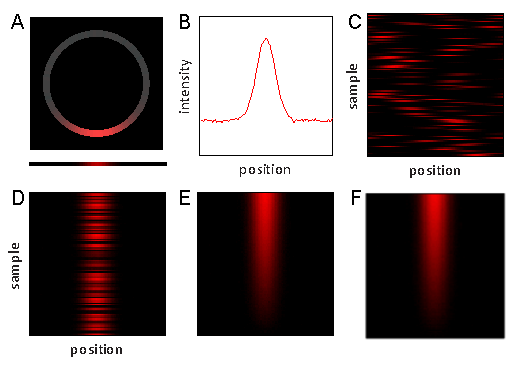
\includegraphics[width=0.7\textwidth]{ch-drosophila/figures/figS2}
\caption[Synthetic data set used to illustrate registration and ordering algorithms]{Synthetic data set used to illustrate the data processing algorithms. (A) One-dimensional concentration profile on a ring (top), and the corresponding profile on a line (bottom). (B) Intensity corresponding to the profile in A. (C) An ensemble of concentration profiles, each of the form described in A. Each row in the array corresponds to a single profile. {(D)} The profiles in {C}, now registered using angular synchronization. {(E)} The profiles in {D}, now temporally ordered using diffusion maps.  {(F)} The profiles in {C}, registered and temporally ordered in a single step using vector diffusion maps.}
\label{fig:1d_demo}
%\customlabel{subfig:1d_example}{\ref{fig:1d_demo}{\it A}}
%\customlabel{subfig:1d_intensity}{\ref{fig:1d_demo}{\it B}}
%\customlabel{subfig:1d_unaligned_unordered}{\ref{fig:1d_demo}{\it C}}
%\customlabel{subfig:1d_aligned_unordered}{\ref{fig:1d_demo}{\it D}}
%\customlabel{subfig:1d_aligned_ordered}{\ref{fig:1d_demo}{\it E}}
%\customlabel{subfig:1d_aligned_ordered_vdm}{\ref{fig:1d_demo}{\it F}}
\end{figure}

The angular synchronization algorithm aligns pairs of data points with respect to a given symmetry group from pairs of alignment measurements \citep{singer2011angular}. 
%
Let $ \data(1), \dots, \data(\ndata)$ denote the signals that we wish to align with respect to rotations;
each signal is a function defined on the unit circle (on the plane).
%
First assume that each signal $\data(i)$ is a {\it noisy} rotated copy of the underlying signal $\data_{true}$
(which we are {\it not} given), such that
\begin{equation}
\data(i) = f(\data_{true}, \theta_i) + \mathbf{\xi}(i)
\end{equation}
where the function $f(\data_{true}, \theta_i)$ rotates the signal $\data_{true}$ by $\theta_i$ degrees, and $\mathbf{\xi}_i$ is a (typically Gaussian) noise term.
%
Our goal is to recover $\theta_1, \dots, \theta_\ndata$.
%
Up to noise,
\begin{equation} \label{eq:pairwise_rot}
\data(i) \approx f(\data(j), \theta_i - \theta_j) ;
\end{equation}
note that \eqref{eq:pairwise_rot} does not require knowledge of $\data_{true}$.
%
We can obtain an {\it estimate} of $\theta_i - \theta_j$ by computing the rotation that optimally aligns $\data(j)$ to $\data(i)$,
i.e., %$\theta_{ij} \approx \theta_i - \theta_j$, where
%
\begin{equation} \label{eq:opt_angle}
\theta_i - \theta_j \approx \theta_{ij} = \argmin_{\theta} \|\data(i) - f(\data(j), \theta)\|^2.
\end{equation}
%
Practically, the signals are discretized in a $\highdim$-long vector (the local intensity at $n$ equidistant points around the circle);
rotating the function by an angle $\theta$ then corresponds to cyclically shifting the elements of $\data(i)$
by $\frac{\theta_i}{2 \pi} \highdim$ (rounded to the nearest integer to obtain a valid shift).
%
For the one-dimensional discretized profiles shown in \fig~\ref{fig:1d_demo}, we exhaustively search over all $\highdim=100$ possible shifts of the signals to obtain the optimal angles in \eqref{eq:opt_angle}.
%
Alternatively, for continuous signals, an optimization algorithm
can be used \citep{ahuja2007template}.

Rather than work with the angles $\theta_{ij}$ directly, it is more convenient to consider the rotation matrices,
\begin{equation} \label{eq:R_theta}
\mathbf{R}(\theta_{ij}) = \begin{bmatrix}
\cos(\theta_{ij}) & -\sin(\theta_{ij}) \\
\sin(\theta_{ij}) & \cos(\theta_{ij})
\end{bmatrix},
\end{equation}
which we can think of as operating on the points of the unit circle (on the plane) on which our signal is defined.
%
Successive rotations correspond to multiplication of the corresponding rotation matrices: $\mathbf{R}(\gamma_1 + \gamma_2) = \mathbf{R}(\gamma_1) \mathbf{R}(\gamma_2)$.
%
Due to the orthogonality of rotation matrices, $\mathbf{R}(-\gamma) = \mathbf{R}(\gamma)^T$.

Let $\rotdim$ denote the dimension of the rotation matrices we are considering (for planar rotations, $\mathbf{R}(\theta_{ij}) \in \mathbb{R}^{2 \times 2}$ and $\rotdim=2$).
%
We construct the matrix $\mathbf{H} \in \mathbb{R}^{\ndata \rotdim \times \ndata \rotdim}$, where $\mathbf{H}$ is an $m \times m$ matrix of $\rotdim \times \rotdim$ blocks, with the $i,j^{th}$ block of $\mathbf{H}$, $\mathbf{H}_{ij}$, defined as
\begin{equation} \label{eq:H_to_R}
\mathbf{H}_{ij} = \mathbf{R}(\theta_{ij}).
\end{equation}
%
%
Under our assumption that $\theta_{ij} \approx \theta_i - \theta_j$, $\mathbf{H}_{ij} \approx \mathbf{R}(\theta_i) \mathbf{R}(\theta_j)^T$
%\begin{equation}
%H_{ij} = R(\theta_{ij}) \approx R(\theta_i - \theta_j) = R(\theta_i) R(-\theta_j) = R(\theta_i) R(\theta_j)^T,
%\end{equation}
 and
\begin{equation} \label{eq:H_low_rank}
	\mathbf{H} \approx
	\begin{bmatrix}
	\mathbf{R}(\theta_1) \\
	\mathbf{R}(\theta_2) \\
	\vdots \\
	\mathbf{R}(\theta_\ndata)
	\end{bmatrix}
	\begin{bmatrix}
	\mathbf{R}(\theta_1)^T \mathbf{R}(\theta_2)^T \dots \mathbf{R}(\theta_\ndata)^T
	\end{bmatrix}.
\end{equation}
%
It follows directly from \eqref{eq:H_low_rank} that the top block eigenvector of $\mathbf{H}$ contains our best estimates of $\mathbf{R}(\theta_1), \mathbf{R}(\theta_2), \dots, \mathbf{R}(\theta_m)$.
%
Let $\phi_0, \phi_1, \dots, \phi_{\ndata \rotdim-1}$ denote the eigenvectors of $\mathbf{H}$ ordered so that $|\lambda_0| \ge |\lambda_1| \ge \dots \ge |\lambda_{\ndata \rotdim -1}|$, where $\lambda_i$ is the eigenvalue corresponding to $\phi_i$.
%
Then,
\begin{equation} \label{eq:R_hat}
\hat{\mathbf{R}} =
\begin{bmatrix}
\hat{\mathbf{R}}_1 \\
\hat{\mathbf{R}}_2 \\
\vdots \\
\hat{\mathbf{R}}_\ndata
\end{bmatrix} =
\begin{bmatrix}
| & | & & | \\
\phi_0 & \phi_1 & \dots & \phi_{\rotdim-1} \\
| & | & & |
\end{bmatrix},
\end{equation}
where $\hat{\mathbf{R}}_i \in \mathbb{R}^{\rotdim \times \rotdim}$ is (nearly) the estimate for $\mathbf{R}(\theta_i)$.
%
To obtain our estimate of $\mathbf{R}(\theta_i$), denoted $\mathbf{R}_{i, est}$, we project $\hat{\mathbf{R}}_i$ onto the closest orthogonal matrix,
\begin{equation} \label{eq:R_est}
\mathbf{R}_{i, est} = \mathbf{U}_i \mathbf{V}_i^T,
\end{equation}
where $\mathbf{U}_i$ and $\mathbf{V}_i$ are the left and right singular vectors, respectively, of $\hat{\mathbf{R}}_i$.
%
We adjust the sign of $\phi_1$ so that $det(\mathbf{R}_{i, est}) = +1$, ensuring proper rotations 
(note that systematically incorporating improper rotations is also possible \citep{goemans1995improved, bandeira2013cheeger}).
%
We estimate $\theta_{i}$ by inverting \eqref{eq:R_theta}, and register the signals by rotating signal $i$ by $-\theta_i$.
%
We note that, in our actual computations, the pairwise rotations $\theta_{ij}$ are computed in a discrete setting, then the overall
synchronization is performed in the continuum context to obtain $\theta_i$, and the results are rounded to give the closest
discrete shift.

Importantly, this formulation also considers {\it higher-order} consistency information.
%
For example, given our pairwise estimates $\mathbf{R}_{ij}$, we know that relationships of the form
\begin{equation} \label{eq:triplet_consistency}
\mathbf{R}(\theta_{ik}) \mathbf{R}(\theta_{kj}) \approx \mathbf{R}(\theta_i) \mathbf{R}(\theta_k)^T \mathbf{R}(\theta_k) \mathbf{R}(\theta_j)^T = \mathbf{R}(\theta_i) \mathbf{R}(\theta_j)^T
\end{equation}
should also hold.
%
Note that
\begin{equation}
(\mathbf{H}^2)_{ij} = \sum_k \mathbf{R}(\theta_{ik}) \mathbf{R}(\theta_{kj});
\end{equation}
therefore, {\it all} information of the form in \eqref{eq:triplet_consistency} is contained in the matrix $\mathbf{H}^2$ (and higher order
consistency information in its higher powers).
%
Because $\mathbf{H}$ and $\mathbf{H}^2$ have the same eigenvectors, our problem formulation accounts for not only pairwise alignment information, but also these higher-order considerations.

\section{Vector Diffusion Maps}

Vector diffusion maps combines the algorithms of angular synchronization and diffusion maps into a single computation that both removes rotational symmetries and parameterizes the data {\em modulo} these symmetries \cite{singer2012vector}.
%
Given data points $\data(1), \dots, \data(\ndata)$, one first constructs the matrix $\mathbf{S} \in \mathbb{R}^{\ndata \rotdim \times \ndata \rotdim}$, with the $i,j^{th}$ block of $\mathbf{S}$, $\mathbf{S}_{ij}$, defined as
\begin{equation} \label{eq:vdm_S}
	\mathbf{S}_{ij} = \mathbf{A}_{ij} \mathbf{H}_{ij}
\end{equation}
%
where $\mathbf{A}_{ij} \in \mathbb{R}$ (defined in \sec~\ref{sec:dmaps}) pertains to the diffusion kernel between data points, and $\mathbf{H}_{ij} \in \mathbb{R}^{\rotdim \times \rotdim}$ (defined in \eqref{eq:H_to_R}) pertains to the pairwise alignment between data points.
%
It is important to note that distance $\| \data(i) - \data(j) \|$ used in the diffusion kernel in \eqref{eq:W} is the distance between data points {\it after} after pairwise alignment, i.e., the minimum distance between all possible shifts of the two data points.
%
In the language of symmetry groups, this distance is a metric between the orbits induced by the relevant symmetry group.

One then computes the eigenvalues $\lambda_0, \lambda_1, \dots, \lambda_{\ndata \rotdim-1}$ and eigenvectors $\phi_0, \allowbreak \phi_1, \dots, \allowbreak \phi_{\ndata \rotdim-1}$ of $\mathbf{S}$, ordered such that $|\lambda_0| \ge |\lambda_1| \ge \dots \ge |\lambda_{\ndata \rotdim-1}|$.
%
These eigenvectors contain information about {\it both} the optimal rotations (the ``synchronization" component) and the
variation of the data {\it after} the spatial symmetries have been removed.
%
Assuming that the data (after symmetries have been factored out) are relatively closely clustered, it is reasonable
to expect, as in angular synchronization, that the top (block) eigenvector of $\mathbf{S}$ contains approximations of the optimal rotations,
which can be computed in the same way from \eqref{eq:R_est}.
%
We then expect subsequent eigenvectors to contain information about the main direction(s) of data variability modulo the geometric symmetries.

In general, the embedding coordinates are given by
\begin{equation} \label{eq:vdm_coord}
\psi_{k,l} (i) = \langle \phi_k(i), \phi_l(i) \rangle,
\end{equation}
where $\phi_k(i) \in \mathbb{R}^{\rotdim}$ denotes the $i^{th}$ block of $\phi_k$,
%
If we assume that the rotations and the dynamics are uncoupled and therefore separable, then the eigenvectors of $\mathbf{S}$ have the following structure: each block eigenvector contains estimates of the optimal rotations (up to a constant rotation) multiplied by the corresponding embedding coordinate (a scalar)
%
As the first diffusion maps coordinate is constant over the data, the first block eigenvector contains only the optimal rotations.
%
The second block eigenvector (eigenvectors $\rotdim$ through $2\rotdim-1$) contains the optimal rotations, each multiplied by their second diffusion maps coordinate.
%
We can therefore recover this diffusion maps coordinate by taking inner products of the columns of the second block eigenvector with columns of the first block eigenvector.
%
The $j^{th}$ embedding coordinate will be given by $\psi_{k,l}$, where $j\rotdim  < k \le (j+1)\rotdim-1$ and $0 \le l \le \rotdim-1$,
and we select $k, l$ such that the coordinate $\psi_{k, l}$ has the largest variability, i.e., the $j^{th}$ coordinate is $\psi_{k,l}$, where $k, l$ is the solution to
\begin{equation} \label{eq:first_embed_vdm}
\max_{
\begin{matrix}
j\rotdim \le k \le (j+1)\rotdim-1 \\
0 \le l \le \rotdim-1
\end{matrix}}
 \sum_i \psi_{k,l} (i)^2. 
\end{equation}

%\section{The eigenvalue spectrum}

We can use the eigenvalues from vector diffusion maps to help deduce the dimensionality of the data.
%
In diffusion maps, the largest eigenvalue will always be 1 and correspond to the trivial (constant) eigenvector, and $|\lambda_k|$ gives a measure of the importance of coordinate $\phi_k$. 
%
We therefore expect to see a ``spectral gap'' in the eigenvalues which separates the meaningful coordinates from those corresponding to noise (modulo higher harmonics; see \chap~\ref{ch:harmonics} and \citep{ferguson2010systematic}).
%
In vector diffusion maps, the importance of each coordinate is measured by the product of the corresponding eigenvalues (i.e., the importance of $\psi_{k,l}$ is given by $| \lambda_k \lambda_l |$). 
%
We again expect to see a ``spectral gap'' in these eigenvalue products between those corresponding to meaningful coordinates (again, modulo higher harmonics) and those corresponding to noise. 